\documentclass[12pt,a4paper,twoside,english,final]{ETHthesis}

% !TEX root = main.tex
\usepackage{ETHthesis}
\usepackage[english]{babel}

% Fonts
\usepackage[T1]{fontenc}
\usepackage[utf8]{inputenc}
\usepackage{lmodern}
\usepackage[usenames, dvipsnames]{xcolor}
\usepackage[dottedtoc,floatperchapter,parts]{classicthesis}

% \usepackage[showframe]{geometry} # Useful to check hbox issues
\usepackage{amsmath, amssymb, amsthm}

% Biblio
\usepackage{csquotes}
\usepackage[backend=bibtex,
            style=alphabetic, natbib=true, url=false,
            isbn=false, backref=true, maxcitenames=3,
            maxbibnames=35]{biblatex}

\usepackage[labelfont=bf]{caption}
\usepackage{subcaption}
\usepackage{tikz}
\usepackage{bbm}
\usepackage{dsfont}
\usepackage{mathtools}
\usepackage{graphicx}

% Tables
\usepackage{tabularx}
\usepackage{booktabs}

% Algorithms
\usepackage[noend]{algpseudocode}
\usepackage{algorithm,algorithmicx}
\usepackage{eqparbox}
\usepackage{xspace}

\usepackage{enumitem}
\setlist[enumerate]{leftmargin=*}

\usepackage{titlesec}
\usepackage{hyperref}
\hypersetup{pdfauthor={Mikhail Karasikov}, pdftitle={}, pdfsubject={A thesis submitted to attain the degree of Doctor of Sciences to ETH Zurich},
            pdflang={en}, bookmarksnumbered, pageanchor=true, plainpages=false, colorlinks=true, linktocpage=true,
            citecolor=MidnightBlue, filecolor=BrickRed, linkcolor=NavyBlue, urlcolor=ForestGreen}

\definecolor{light-gray}{gray}{0.65}
\titleformat{\chapter}% Command
[display]% shape
{\bfseries\Large}% Format for the whole title
{\filleft{\fontsize{80}{100}\selectfont\color{light-gray}\thechapter}}% Label
{-25pt}% horizontal separation (vertical for display)
{\filleft\fontsize{26}{35}\selectfont}% Before Code
[\vspace{5pt}\titlerule]

%% Page Layout
\setlength{\topmargin}{-7.5mm}
\setlength{\headheight}{5mm}
\setlength{\headsep}{+12.5mm}
\setlength{\textheight}{220mm}
\setlength{\footskip}{+20.mm}
\setlength{\textwidth}{161mm} %!!!
\setlength{\parindent}{0pt}
\setlength{\parskip}{1ex plus 0.25ex minus 0.25ex}
\iftwoside
\setlength{\oddsidemargin}{3mm}
\setlength{\evensidemargin}{-3mm}
\else
\setlength{\oddsidemargin}{0mm}
\setlength{\evensidemargin}{0mm}
\fi
\raggedbottom

%% Float Placement
\renewcommand{\topfraction}{0.85}
\renewcommand{\bottomfraction}{0.85}
\renewcommand{\textfraction}{0.15}
\renewcommand{\floatpagefraction}{0.1}
\renewcommand{\baselinestretch}{1.15}

% Allow subsubsections to have numbers (and be references)
\setcounter{secnumdepth}{3}
% Allow subsubsections to appear in the TOC
\setcounter{tocdepth}{3}
% \setcounter{lofdepth}{2} % we want subfigures in the list of figures

%% Line spacing
\linespread{1.25}

%% Avoid Widows and Orphans
\widowpenalty=1000
\clubpenalty=1000

\vfuzz2pt % Don't report over-full v-boxes if over-edge is small
\hfuzz2pt % Don't report over-full h-boxes if over-edge is smallq

% !TEX root = main.tex
% Allow overfull boxes which don't overflow more than 20pts (remove before the last version)
\hfuzz=20pt

% Issue with transparency of included pdf images (if there is more than 1 per page with \group
% defined pdflatex doesn't know which one to consider the top one ...)
\pdfsuppresswarningpagegroup=1

\newcommand{\cleardoublepageempty}{
  \clearpage
  \thispagestyle{empty}
  \cleardoublepage
}

\usepackage{array}
\newcolumntype{H}{>{\setbox0=\hbox\bgroup}c<{\egroup}@{}} % Useful to hide a column of a table (just define it as H)

\newtheorem*{rep@theorem}{\rep@title}
\newcommand{\newreptheorem}[2]{%
\newenvironment{rep#1}[1]{%
 \def\rep@title{#2 \ref{##1}}%
 \begin{rep@theorem}}%
 {\end{rep@theorem}}}
\newreptheorem{lemma}{Lemma'}
\newreptheorem{theorem}{Theorem'}
\newreptheorem{corollary}{Corollary'}
\newtheorem{theorem}{Theorem}
\newtheorem{lemma}[theorem]{Lemma}
\newtheorem{corollary}[theorem]{Corollary}
\newtheorem{definition}[theorem]{Definition}
\newtheorem{proposition}[theorem]{Proposition}
\makeatletter
\@addtoreset{theorem}{chapter}
\makeatother

\newcommand{\mop}[1]{\mathop{\text{#1}}}

\makeatletter
\DeclareRobustCommand\bfseries{%
  \not@math@alphabet\bfseries\mathbf
  \fontseries\bfdefault\selectfont
  \boldmath % <-- added
}
\makeatother
% !TEX root = main.tex
\usepackage{url}            % simple URL typesetting
\usepackage{amsfonts}       % blackboard math symbols
\usepackage{nicefrac}       % compact symbols for 1/2, etc.
\usepackage{microtype}      % microtypography
\usepackage{amsbsy}%
\usepackage{calc}
\usepackage{moresize}
\usepackage{siunitx}
\usepackage{bm}
\usepackage{multirow}
\usepackage{printlen}
\newtheorem{assu}{Assumption}
\newtheorem{remark}{Remark}

\usepackage{multicol}
\usepackage{footmisc}
\usetikzlibrary{positioning, matrix, shapes,trees}
\usepackage{mathtools}
\usepackage[export]{adjustbox}
\usepackage{wrapfig}
\usepackage[outdir=./]{epstopdf}
\usepackage[sort=def]{glossaries}

% \usepackage{sistyle}
% \SIthousandsep{,}
%\usepackage{breqn}


\makeatletter
\makeatother

\usepackage{tikz}
\usetikzlibrary{calc}
\tikzset{mynode/.style={draw,circle, minimum size = 0.7cm}}
\usetikzlibrary{positioning,shapes,arrows}
\usepackage{xcolor}

\definecolor{gblue}{RGB}{207,226,243}
\definecolor{gred}{RGB}{244,204,204}
\definecolor{gyellow}{RGB}{255,229,153}
\definecolor{gyellow2}{RGB}{252,229,205}
\definecolor{ggreen}{RGB}{217,234,211}
\definecolor{ggray}{RGB}{238,238,238} 
\definecolor{ggray2}{RGB}{81,84,87} 
\definecolor{gpurple}{RGB}{217,210,233} 

\usepackage{anyfontsize}

% \usepackage{forest}
% \definecolor{folderbg}{RGB}{124,166,198}
% \definecolor{folderborder}{RGB}{110,144,169}
% \def\Size{4pt}
% \tikzset{
%   folder/.pic={
%     \filldraw[draw=folderborder,top color=folderbg!50,bottom color=folderbg]
%       (-1.05*\Size,0.2\Size+5pt) rectangle ++(.75*\Size,-0.2\Size-5pt);
%     \filldraw[draw=folderborder,top color=folderbg!50,bottom color=folderbg]
%       (-1.15*\Size,-\Size) rectangle (1.15*\Size,\Size);
%   }
% }

\usepackage{listings}

\usepackage{tabularray}

% !TEX root = main.tex

%%%%%%%%%%%%%%%%%%%%%%%%%%%%%%%%%%%%%%%%%%%%%%%%%%%%%%%%%%%%%%%%%%%%%%%%%%%%%%%
% Overall commands
%%%%%%%%%%%%%%%%%%%%%%%%%%%%%%%%%%%%%%%%%%%%%%%%%%%%%%%%%%%%%%%%%%%%%%%%%%%%%%%
% Comments
\newcommand{\FL}[1]{{\textcolor{blue}{{\bf FL:} #1}}}

% Common expressions
\newcommand{\ie}{\textit{i.e.}\xspace}
\newcommand{\eg}{\textit{e.g.}\xspace}
\newcommand{\iid}{\textit{i.i.d.}\xspace}

% Full citations
\makeatletter
\newcommand{\upmax}{\def\blx@maxcitenames{99}}
\newcommand{\dnmax}{\def\blx@maxcitenames{1}}
\makeatother
\newcommand{\myfullcite}[1]{\upmax\fullcite{#1}\dnmax}

%%%%%%%%%%%%%%%%%%%%%%%%%%%%%%%%%%%%%%%%%%%%%%%%%%%%%%%%%%%%%%%%%%%%%%%%%%%%%%%
% MAIN BACKGROUND
%%%%%%%%%%%%%%%%%%%%%%%%%%%%%%%%%%%%%%%%%%%%%%%%%%%%%%%%%%%%%%%%%%%%%%%%%%%%%%%

% Big-O notation
\newcommand{\Or}[1]{\mathcal{O}\mathopen{}\left(#1\right)\mathclose{}}
\newcommand{\OrTilde}[1]{\tilde{\mathcal{O}}\mathopen{}\left(#1\right)\mathclose{}}
\newcommand{\Th}[1]{\Theta\mathopen{}\left(#1\right)\mathclose{}}
\newcommand{\Om}[1]{\Omega\mathopen{}\left(#1\right)\mathclose{}}

\newcommand{\encase}[1]{{\left[#1\right]}}
\newcommand{\brac}[1]{{\left(#1\right)}}


% Real numbers
\newcommand{\R}{\mathbb{R}}
\newcommand{\N}{\mathbb{N}}

% Optimization notation
\newcommand{\trace}{\operatorname{tr}}
\newcommand{\dist}{\operatorname{dist}}
\newcommand{\norm}[1]{\Vert #1 \Vert}
\newcommand{\ip}[2]{\big\langle #1, \, #2 \big\rangle}
\newcommand{\prox}[1]{\mathrm{prox}_{#1}}
\newcommand{\proj}[1]{\mathrm{proj}_{#1}}
\newcommand{\lmo}{\textit{lmo}\xspace}
\def\bbE{{\mathbb{E}}}
\def\E{{\mathbb{E}}}
\def\sR{{\mathbb{R}}}
\def\sZ{{\mathbb{Z}}}

\DeclareMathOperator*{\argmin}{arg\,min}
\DeclareMathOperator*{\argmax}{arg\,max}

% Optimization problems
\DeclareMathOperator{\conv}{conv}
\DeclareMathOperator{\lin}{lin}
\DeclareMathOperator{\cone}{cone}

% VI Commands
\newcommand{\dkl}{D^{KL}}
\newcommand{\KL}{D^{KL}}
\newcommand{\relbo}{\textsc{RELBO}\xspace}


% Algorithms
\newcommand{\FW}{{\textsf{\tiny FW}}}


\DeclareMathOperator{\l1}{L1-ball}
\DeclareMathOperator{\Cf}{C_f}
\DeclareMathOperator{\radius}{\mathrm{radius}}
\DeclareMathOperator{\diam}{\mathrm{diam}}
\DeclareMathOperator{\mdw}{mDW(\cA)}
\DeclareMathOperator{\ama}{{\cA\cup-\cA}}
\DeclareMathOperator{\amx}{\left\lbrace\cA\cup-\frac{\theta_k}{\|\theta_k\|_\cA}\right\rbrace}
\DeclareMathOperator{\amxnok}{\left\lbrace\cA\cup-\frac{\theta}{\|\theta\|_\cA}\right\rbrace}
\DeclareMathOperator{\faces}{faces}
\DeclareMathOperator{\gfaces}{g-faces}
\DeclareMathOperator{\madw}{mADW(\cA)}
\DeclareMathOperator{\cw}{CWidth(\cA)}
\DeclareMathOperator{\clip}{clip}

% Matchal laetters
\def\cA{\mathcal{A}}
\def\cB{\mathcal{B}}
\def\cD{\mathcal{D}}
\def\cF{\mathcal{F}}
\def\cH{\mathcal{H}}
\def\cK{\mathcal{K}}
\def\cL{\mathcal{L}}
\def\cN{\mathcal{N}}
\def\cQ{\mathcal{Q}}
\def\cS{\mathcal{S}}
\def\cT{\mathcal{T}}
\def\cZ{\mathcal{Z}}

% Random Variables
\def\rva{{\mathbf{a}}}
\def\rvb{{\mathbf{b}}}
\def\rvc{{\mathbf{c}}}
\def\rvd{{\mathbf{d}}}
\def\rve{{\mathbf{e}}}
\def\rvf{{\mathbf{f}}}
\def\rvg{{\mathbf{g}}}
\def\rvh{{\mathbf{h}}}
\def\rvu{{\mathbf{i}}}
\def\rvj{{\mathbf{j}}}
\def\rvk{{\mathbf{k}}}
\def\rvl{{\mathbf{l}}}
\def\rvm{{\mathbf{m}}}
\def\rvn{{\mathbf{n}}}
\def\rvo{{\mathbf{o}}}
\def\rvp{{\mathbf{p}}}
\def\rvq{{\mathbf{q}}}
\def\rvr{{\mathbf{r}}}
\def\rvs{{\mathbf{s}}}
\def\rvt{{\mathbf{t}}}
\def\rvu{{\mathbf{u}}}
\def\rvv{{\mathbf{v}}}
\def\rvw{{\mathbf{w}}}
\def\rvx{{\mathbf{x}}}
\def\rvy{{\mathbf{y}}}
\def\rvz{{\mathbf{z}}}

\def\sfA{\mathsf{A}}
\def\sfQ{\mathsf{Q}}
\def\sfZ{\mathsf{Z}}

% Random variables
\def\reta{{\textnormal{$\eta$}}}
\def\ra{{\textnormal{a}}}
\def\rb{{\textnormal{b}}}
\def\rc{{\textnormal{c}}}
\def\rd{{\textnormal{d}}}
\def\re{{\textnormal{e}}}
\def\rf{{\textnormal{f}}}
\def\rg{{\textnormal{g}}}
\def\rh{{\textnormal{h}}}
\def\ri{{\textnormal{i}}}
\def\rj{{\textnormal{j}}}
\def\rk{{\textnormal{k}}}
\def\rl{{\textnormal{l}}}
% rm is already a command, just don't name any random variables m
\def\rn{{\textnormal{n}}}
\def\ro{{\textnormal{o}}}
\def\rp{{\textnormal{p}}}
\def\rq{{\textnormal{q}}}
\def\rr{{\textnormal{r}}}
\def\rs{{\textnormal{s}}}
\def\rt{{\textnormal{t}}}
\def\ru{{\textnormal{u}}}
\def\rv{{\textnormal{v}}}
\def\rw{{\textnormal{w}}}
\def\rx{{\textnormal{x}}}
\def\ry{{\textnormal{y}}}
\def\rz{{\textnormal{z}}}


\def\va{{\textbf{a}}}
\def\vb{{\textbf{b}}}
\def\vc{{\textbf{c}}}
\def\vd{{\textbf{d}}}
\def\ve{{\textbf{e}}}
\def\vf{{\textbf{f}}}
\def\vg{{\textbf{g}}}
\def\vh{{\textbf{h}}}
\def\vi{{\textbf{i}}}
\def\vj{{\textbf{j}}}
\def\vk{{\textbf{k}}}
\def\vl{{\textbf{l}}}
\def\vm{{\textbf{m}}}
\def\vn{{\textbf{n}}}
\def\vo{{\textbf{o}}}
\def\vp{{\textbf{p}}}
\def\vq{{\textbf{q}}}
\def\vr{{\textbf{r}}}
\def\vs{{\textbf{s}}}
\def\vt{{\textbf{t}}}
\def\vu{{\textbf{u}}}
\def\vv{{\textbf{v}}}
\def\vw{{\textbf{w}}}
\def\vx{{\textbf{x}}}
\def\vy{{\textbf{y}}}
\def\vz{{\textbf{z}}}

% Matrix
\def\mA{{\textbf{A}}}
\def\mB{{\textbf{B}}}
\def\mC{{\textbf{C}}}
\def\mD{{\textbf{D}}}
\def\mE{{\textbf{E}}}
\def\mF{{\textbf{F}}}
\def\mG{{\textbf{G}}}
\def\mH{{\textbf{H}}}
\def\mI{{\textbf{I}}}
\def\mJ{{\textbf{J}}}
\def\mK{{\textbf{K}}}
\def\mL{{\textbf{L}}}
\def\mM{{\textbf{M}}}
\def\mN{{\textbf{N}}}
\def\mO{{\textbf{O}}}
\def\mP{{\textbf{P}}}
\def\mQ{{\textbf{Q}}}
\def\mR{{\textbf{R}}}
\def\mS{{\textbf{S}}}
\def\mT{{\textbf{T}}}
\def\mU{{\textbf{U}}}
\def\mV{{\textbf{V}}}
\def\mW{{\textbf{W}}}
\def\mX{{\textbf{X}}}
\def\mY{{\textbf{Y}}}
\def\mZ{{\textbf{Z}}}

\def\gA{{\mathcal{A}}}
\def\gB{{\mathcal{B}}}
\def\gC{{\mathcal{C}}}
\def\gD{{\mathcal{D}}}
\def\gE{{\mathcal{E}}}
\def\gF{{\mathcal{F}}}
\def\gG{{\mathcal{G}}}
\def\gH{{\mathcal{H}}}
\def\gI{{\mathcal{I}}}
\def\gJ{{\mathcal{J}}}
\def\gK{{\mathcal{K}}}
\def\gL{{\mathcal{L}}}
\def\gM{{\mathcal{M}}}
\def\gN{{\mathcal{N}}}
\def\gO{{\mathcal{O}}}
\def\gP{{\mathcal{P}}}
\def\gQ{{\mathcal{Q}}}
\def\gR{{\mathcal{R}}}
\def\gS{{\mathcal{S}}}
\def\gT{{\mathcal{T}}}
\def\gU{{\mathcal{U}}}
\def\gV{{\mathcal{V}}}
\def\gW{{\mathcal{W}}}
\def\gX{{\mathcal{X}}}
\def\gY{{\mathcal{Y}}}
\def\gZ{{\mathcal{Z}}}


\renewcommand{\P}{P}
\newcommand{\Q}{Q}

\DeclareRobustCommand{\myhammer}{%
  \begingroup\normalfont
  \includegraphics[height=1.1\fontcharht\font`\B]{sections/disent/figures/hammer.pdf}%
  \endgroup
}
\newcommand{\PA}{\textbf{PA}}
\newcommand{\supp}{\operatorname{supp}}

\newcommand\blfootnote[1]{%
  \begingroup
  \renewcommand\thefootnote{}\footnote{#1}%
  \addtocounter{footnote}{-1}%
  \endgroup
}


\newcommand{\softmax}[1]{\texttt{Softmax}\,(#1)}
\newcommand{\dotp}[1]{\texttt{dot}\,(#1)}
\newcommand{\reducesum}[1]{\texttt{reduce\_sum}\,(#1)}
\newcommand{\gru}[2]{\texttt{GRU}\,(#1, \ #2)}
\newcommand{\slots}[0]{\texttt{slots}}
\newcommand{\attn}[0]{\texttt{attn}}
\newcommand{\inp}[0]{\texttt{inputs}}
\newcommand{\mlp}[0]{\texttt{MLP}}
\newcommand{\sam}[0]{Slot Attention\xspace}
\newcommand{\w}[0]{\texttt{w}}
\newcommand{\updates}[0]{\texttt{updates}}
\newcommand{\layernorm}[0]{\texttt{LayerNorm}}
\newcommand\myeq{\mkern0.5mu{=}\mkern6mu}
% \renewcommand{\algorithmiccomment}[1]{#1}

\DeclareMathOperator{\rank}{rank}
\DeclareMathOperator{\select}{select}
\newcommand{\kmer}{\operatorname{\text{k-mer}}}

\makeatletter\renewcommand{\ALG@beginalgorithmic}{\small}\makeatother
\newcommand*\Let[2]{#1 $\gets$ #2}
\algnewcommand{\LineComment}[1]{\State \(\triangleright\) #1}
\algrenewcommand\algorithmicrequire{\textbf{Precondition:}}
\algrenewcommand\algorithmicensure{\textbf{Postcondition:}}
% declaration of the new block
% \algblock{ParFor}{EndParFor}
% customising the new block
% \algnewcommand\algorithmicparfor{\textbf{parfor}}
\algnewcommand\algorithmicpardo{\textbf{do}}
% \algnewcommand\algorithmicendparfor{\textbf{end\ parfor}}
% \algrenewtext{ParFor}[1]{\algorithmicparfor\ #1\ \algorithmicpardo}
% \algrenewtext{EndParFor}{\algorithmicendparfor}

% declaration of the new block
\algblock{ParForAll}{EndParForAll}
% customising the new block
\algnewcommand\algorithmicparforall{\textbf{for all}}
\algnewcommand\algorithmicparforalldo{\textbf{parallel do}}
\algrenewtext{ParForAll}[1]{\algorithmicparforall\ #1\ \algorithmicparforalldo}
\algtext*{EndParForAll}%

\def\code#1{\texttt{#1}}


\bibliography{ref}


% !TEX root = ./main.tex

\makenoidxglossaries

\newglossaryentry{dna_sequencing}{
	name={DNA sequencing},
	description={The process of inferring the nucleic acid sequence, the nucleotides in DNA. There are different methods or {\em technologies} used to perform this process and determine the sequence of the four nucleotides: adenine (A), guanine (G), cytosine (C), and thymine (T) in the sequenced DNA molecule}
}


\begin{document}
\initETHthesis

%%%%%%%%%%%%%%%%%%%%%%%%%%%%%%%%%%%%%%%%
% COVER PAGE %
%%%%%%%%%%%%%%%%%%%%%%%%%%%%%%%%%%%%%%%%
\dissnum{$000000$}
\title{Learning to align single-cell populations}
\author{Stefan Stark}
% \acatitle{\normalsize M.Sc. in Applied Mathematics and Physics,\\Moscow Institute of Physics and Technology}
\dateofbirth{March $11$, $1992$}
\citizen{United States}
%\date{November 2020}
\Year{2024}
\examiners{
	\normalsize
  Prof.\ Dr.\ Gunnar R\"atsch (ETH Zurich), examiner\linebreak
  Dr.\ Kjong-van Lehmann (RWTH), examiner\linebreak
  Prof. Dr.\ Andreas Krause (ETH Zurich), co-examiner\linebreak
  Prof. Dr.\ Oliver Stegle (EMBL), co-examiner\linebreak
}
\support{}
\disclaimer{}
\pagestyle{empty}
\hypersetup{pageanchor=false}
\maketitle
\hypersetup{pageanchor=true}

%%%%%%%%%%%%%%%%%%%%%%%%%%%%%%%%%%%%%%%%
% PREAMBLE %
%%%%%%%%%%%%%%%%%%%%%%%%%%%%%%%%%%%%%%%%
\pagestyle{plain}
\pagenumbering{roman}
%% !TeX root = ../main.tex

\pdfbookmark[1]{Abstract}{Abstract}
\begingroup
\let\clearpage\relax
\let\cleardoublepage\relax
\let\cleardoublepage\relax

\chapter*{Abstract}
Cellular states are complex -- their underlying genomic sequence, RNA transcription levels, accessibility of chromatin regions, protein levels, chemical activity, etc, work in tandem to determine the behavior of a cell and its responses to changes in its environment. 
Initially, the study of cellular populations relied on bulk profiling technologies
%which average individual cellular signals across population into a single observation, and
that made it difficult to study heterogeneous populations.
However, this last decade has seen, and continues to see, an explosion in the development of single-cell profiling technologies that allow individual cellular states to be observed at scale.
While these technologies revolutionized the study of cellular biology, they are still typically limited in the sense that they consume or otherwise destroy profiled cells.
This means that an individual cell can only be measured once.
As a result, these technologies are only able to measure projections of the underlying \textit{holistic} cellular state into a single observable domain, measuring, for instance, either a cell's RNA transcript abundance or the protein levels.
Furthermore, modeling temporal processes, such as perturbation responses, remain challenging, as these complex behaviors must be recovered without access to some set of paired "input-output" states.

This thesis is broadly concerned with the development and application of machine-learning based methods to reconcile this single-observation limitation.
The typical modern single-cell experiment will generate two (or more) datasets, which we can consider sampled from distributions over cellular states, $\mu$ and $\nu$, that share some non-trivial relationship.
We aim to recover this relationship by learning to \emph{align} these cellular populations.
Specifically we describe how to
i) integrate multi-modal observations, in which $\mu$ and $\nu$ represent the state of population different observable domains
and ii) model perturbation responses of cellular populations, in which $\mu$ and $\nu$ represent population state at two different time points.
A major theme throughout this thesis is the demonstration of clinical utility of the developed methods.
In particular, we apply a method developed to recover and predict heterogeneous single-cell responses to a cohort of melanoma patients and demonstrate how it can improve the analysis, understanding, and ultimately help tailor their treatments.




\newpage
\begin{otherlanguage}{ngerman}
\pdfbookmark[1]{Zusammenfassung}{Zusammenfassung}
\chapter*{Zusammenfassung}
% TODO: (later) translate abstract
[german translation]
\end{otherlanguage}


%\newpage
%\chapter*{Acknowledgments}
% TODO: (later) write awks
\endgroup

\vfill

\cleardoublepageempty{}
\selectlanguage{english}

%%%%%%%%%%%%%%%%%%%%%%%%%%%%%%%%%%%%%%%%
% TOC %
%%%%%%%%%%%%%%%%%%%%%%%%%%%%%%%%%%%%%%%%
\setlength{\cftbeforechapskip}{4mm}
\setcounter{tocdepth}{1}
\pagestyle{myheadings}
\pdfbookmark[0]{\contentsname}{contents}
\tableofcontents
\cleardoublepageempty{}

%%%%%%%%%%%%%%%%%%%%%%%%%%%%%%%%%%%%%%%%
% GLOSSARY %
%%%%%%%%%%%%%%%%%%%%%%%%%%%%%%%%%%%%%%%%
\printnoidxglossaries
\cleardoublepageempty{}

%%%%%%%%%%%%%%%%%%%%%%%%%%%%%%%%%%%%%%%%
% BODY %
%%%%%%%%%%%%%%%%%%%%%%%%%%%%%%%%%%%%%%%%
\pagenumbering{arabic}
\cleardoublepageempty{}
\chapter{Introduction}
\subsection{Scope}
\subsection{Publications}
\subsection{Collaborators}

\section{Individual cells as complex machinery}
\subsection{central dogma}
\subsection{pathways \& signaling hierarchies}

\section{Single-cell profiling technologies}
\subsection{scRNA-seq}
\subsubsection{autoencoders}
\subsection{proteomic technologies}
\subsubsection{CyTOF}
\subsubsection{4i \& other imaging}
\subsubsection{marker choices}

\section{Casting as alignment}
\subsection{Holistic view of cells}
\subsection{Dynamic processes}
\subsection{The observation problem}

\chapter{Multi-modal integration}
% TODO major: format citations
\section{Background}
The ability to dissect a tissue into its cellular components to study them individually or to investigate the interplay between the different cell type fractions is an exciting new possibility in biological research.
These lines of research have yielded important insights into the dynamics of various diseases, especially for cancer (Chevrier et al., 2017; Tirosh et al., 2016).
Recent advances in single-cell technologies enable molecular profiling of samples with greater granularity at the transcriptomic, proteomic, genomic as well as the functional assays level (Irmisch et al., 2020; Rozenblatt-Rosen et al., 2017).
While each of these data modalities offer insight into different types and levels of internal cellular processes,
a \textit{holistic} understanding of cellular state could be obtained through the combination or integration of these modalities.
Knowing the measurement of multiple modalities for individual cells would deepen our understanding of the cellular mechanisms at play in, for instance, the tissue microenvironment, and construct a comprehensive molecular view of profiled samples.s

A key challenge towards such integration, however, lies in the limitations of profiling technologies.
Since ubiquitous technologies, such as scRNA-seq and CyTOF, consume the profiled cells, it is typically not possible to observe these cells in more than one modality.
While technologies capable of measuring multiple modalities simultaneously are emerging (Stoeckius et al., 2017; Zhu et al., 2020), they remain limited in terms of scalability and practicality.
Thus, the multi-modal integration of cellular processes falls to computational methods.
Given observation datasets across individual profiling modalities, these methods typically assume that the samples profiled in each modality are somehow similar in composition, and perform integration bo constructing and \textit{alignment} across these datasets.
A critical complication towards this alignment lies in the weak correspondences between the feature sets over these modalities
For instance, there does not exist a one-to-one correspondence between genes (as profiled by scRNA-seq) and proteins (as profiled by CyTOF).
Thus, proper alignment is a challenging task.

%\bold{Related work}
While multiple data integration tools have been developed, most approaches either depend on or impose feature correspondences (Stuart et al., 2019; Welch et al., 2019), or are designed to applied to a limited set of modalities, for instance, scRNA and scDNA data (Campbell et al., 2019; McCarthy et al., 2020).
To the best of our knowledge only two other approaches have been published (Amodio and Krishnaswamy, 2018; Welch et al., 2017) able to perform integration over general modalities.
MAGAN (Amodio and Krishnaswamy, 2018) is a Generative Adversarial Network capable of aligning the manifold between two technologies that relies on a feature correspondence loss.
MATCHER (Welch et al., 2017) is based on a Gaussian process latent variable model (GPLVM) (Lawrence, 2004) that can integrate technologies if their underlying latent structures can be represented in one dimension, applicable, for example, to model monotonic temporal processes.
Other yet unpublished methods, such as MMD-MA (Liu et al., 2019) and UnionCom (Cao et al., 2020), rely on large kernel matrices which limit their scalability when using datasets of the sizes generally produced by molecular profiling.

Here, we propose Single-cell Integration via Matching (SCIM), a method to match cells across different single-cell ’omics technologies.
Our approach is universal, in the sense that it is in principle applicable to any single-cell technology and overcomes the scaling issues of contemporary approaches.
Further, we do not assume the existence of paired features between two technologies.
This allows for the integration of technologies that measure for example the expression of a disjoint set of genes, or the integration of gene expression with image features as long as the underlying latent structure is present in those features.

\section{Single-cell integration via Matching}
SCIM achieves multi-modal single-cell integration in two steps.
First, we construct an integrated latent space using an adversarial autoencoder framework (CITE) wherein representations are invariant to their corresponding technologies, inspired by a model proposed previously (Yang and Uhler, 2019) and further extended in Yang et al. (2019).
In the second step, we perform a strong pairwise alignment of datasets from each modality via a cell-to-cell matching strategy that efficiently extracts cross-technology cell matches from the latent space.
SCIM assumes a shared latent representation between technologies but, unlike other approaches, does not require one-to-one or overlapping correspondences between feature sets.
SCIM scales well in the number of cells in the input through the use of neural-nets, end-to-end training and an efficient bipartite matching algorithm.
Finally, this training scheme allows for the addition of an arbitrary number of technologies, which can be trained in parallel.

\subsection{Constructing technology-invariant representations}
SCIM encodes datasets into a shared latent space that is constructed to have two properties:
% TODO minor reference VAE section
First, inputs should be able to be reconstructed from their latent representations, as is typically achieved by vanilla VAEs.
2) the latent representations of each technology should be well-integrated such that they are indistinguishable from each other.
In a successful integration the resulting latent space will have corresponding cells across all technologies represented in close proximity.

To construct an integrated latent space, SCIM uses a modified adversarial auto encoder framework.
% TODO minor: explain source/target modalities
%First, one modality is chosen as the source modality and the other modalities are regarded as the target modalities.
This consists of the following networks: a pair of encoder ($\phi_k$) and decoder ($\psi_k$) networks for each technology $k$ and a single discriminator network ($\gamma$) acting on the latent space.
This discriminator is a binary classifier trained to identify the latent representation of some source technology from latent representations of all other technologies using a binary cross entropy loss.

SCIM yields an integrated latent space by minimizing the reconstruction error while adversarially fooling the discriminator.
Given the measurements of a batch of cells from the target modality $t$, $x_t$, and the (fixed) latent representations of a batch of cells from the source modality $s$, $\hat{z}_s \sim \phi_s(x_s)$,
% TODO major: fix SCIM equations, write as min-max
\begin{equation}
1 = 2
\end{equation}

$\mathcal{L}_{nll}$ is the negative log-likelihood of the inputs under their reconstruction.
$\mathcal{L}_{adv}$ is the discriminator’s classification error when trying to classify the latent representation samples $\hat{z}_s$ or $\hat{z}_t$ as the source or target technology.
$\beta$ is a hyperparameter weighing the influence of the adversarial loss.
%At the same time, c is trained to correct- ly classify the technology of the z^s and z^t samples.

\paragraph{Latent space orientation}
Correctly orienting the latent space in an unsupervised manner is a challenging task (Locatello et al., 2018; Yang and Uhler, 2019).
Consider, for example, a simple monotonic temporal process.
The latent representations for one dataset could be oriented from start to end, while another could be oriented from finish to start (Welch et al., 2017).
% TODO minor: fix eqn ref
Equation 2 is satisfied, the representations are well integrated and inputs can be correctly reconstructed from them, yet the inter-dataset relationships are misaligned.
Makhzani et al. (2015) address a similar problem by concatenating one-hot representations of labels reflecting intra-technology structure (e.g. cell type is an appropriate choice for ’omics datasets) to the discriminator inputs, showing that this supervision is necessary to orient the latent space.
Furthermore, Locatello et al. (2019) argued that only a small number of labels are actually needed to achieve orientation.
To this end, we adopt a semi-supervised approach by adding a ‘censored’ label and randomly relabel cells in the training set.

\paragraph{Model architecture}
Unless specified otherwise, we adopt the following architecture settings.
All networks use the ReLU activation. % TODO minor: cite/ref/describe ReLU?
We set the latent dimension of all models to eight, but observed this choice to be flexible.
We use discriminator networks with two layers and eight hidden units each.
% TODO major: describe spectral norm?
The Spectral Normalization framework (Miyato et al., 2018) is used during training, which has been argued to stabilize discriminator training by effectively bounding its gradients.
We use a Gaussian activation for all decoders, a 2 layer architecture with 64 hidden units for all simulated data networks, a 2 layer architecture with 8 hidden units for all CyTOF networks and a 2 layer architecture with 64 hidden units for all scRNA networks.
The number of features and complexity of data is considered when choosing capacity and depth.

\paragraph{Optimization}
Optimization proceeds by iteratively fixing one technology as the source and one technology as the target.
In the case of more than two technologies, the technology corresponding to the discriminator’s positive class must either be the source or target technology.
Optimization proceeds with an inner and outer loop.
% TODO minor: ref eqn correctly
In a single inner loop step, the latent representations of the source technology are fixed and Equation XX is minimized with gradient updates to the encoder and decoder of the target modality $t$ using gradients computed on the batch $x_t$.
This process is repeated multiple times and then one step of the outer loop is performed.
In a single outer loop step, the discriminator is updated to classify $z_s$ and $z_t$.
All networks are optimized using the ADAM algorithm (Kingma and Ba, 2014).


\paragraph{Model Selection}
Due to the min–max nature of adversarial training, model comparison is challenging since one cannot directly compare the minimized objective functions of converged models (Lucic et al., 2017).
While the computer vision community has introduced a number of metrics specific to the image domain to help compare models (Heusel et al., 2017; Salimans et al., 2016), here we need to validate the quality of a set of lower-dimensional latent representations.
To achieve this, we utilize a k-Nearest Neighbor (kNN)-based divergence estimator (Wang et al., 2009).
The divergence score between two sets of codes $Z_s$ and $Z_t$ is calculated as:
% TODO minor: typeset eqn
\begin{equation}
	a = b
\end{equation}
This estimator approximates a symmetric variant of a KL divergence, a measure of how much two distributions differ, using only empirical data.
The divergence estimate is computed between the latent representations of the source technology and the target technology to measure the alignment of codes from the two technologies.
Model selection can proceed at scale by selecting parameter configurations that align technology distributions and have low reconstruction error.

\subsection{Bipartite matching of single-cell embeddings}
In its second step, SCIM performs multi-modal integration by identifying pairs of corresponding cells across two modalities using their representations in the latent space constructed in the first step.
We identify pairs by solving a combinatorial bipartite matching problem (Ahuja et al., 1993; Dell’Amico and Toth, 2000), wherein the bipartite graph is constructed by connecting cells between each pair of technologies, weighted by their distances in the latent space.
The bipartite matching problem then identifies an optimal set of paired cells that minimizes the total edge cost of all matches.
In order to achieve this efficiently and at scale, we approximate the full bipartite graph with a k-Nearest Neighbors (kNN) graph that identifies a set of potential matches for each cell and reduces the complexity of the problem.
We then extend the graph to account for single-cell data characteristics and solve the bipartite matching within a general framework of Minimum-Cost Maximum-Flow problems (Ahuja et al., 1993; Klein, 1967).

\paragraph{kNN subgraph approximation}
Given the large number of cells in single-cell datasets, we reduce the search space to the $k$ most likely potential matches.
For each pairwise integration task, two kNN graphs are built: the first uses the source data queried by the target technology cells, and the second uses target data queried by the source technology
That is, each cell in the source technology is connected to its $k$ nearest neighbor cells in the target technology and each cell in the target technology is connected to its $k$ nearest neighbor cells in the source technology.
The union of this graph is then used in the bipartite matching solver.
The sparsity of these connections, regulated by the choice of the hyperparameter $k$, corresponds to a trade-off between the computational performance (memory usage, run time) and the final matching accuracy.

%\paragraph{Min\-cost Max\-flow matching}
Based on a Euclidean cost matrix, we aim at finding the maximum number of cell pairs with minimum cost.
This corresponds to finding a maximum flow that can be pushed through the graph, where each edge between cells has capacity 1, while minimizing the overall cost.
To solve the Minimum-Cost Maximum-Flow problem in a compu- tationally efficient way we use an implementation of the network simplex algorithm (Kira ́ly and Kova ́cs, 2012).

















\chapter{Learning perturbation responses}
\section{Related works}
\subsection{Piece-wise linear approximations}
\subsection{Linear shifts in latent space}

\section{Optimal transport}
\subsection{Primal OT formulation}
\subsection{Dual OT formulation}
\subsection{Neural optimal transport}
\subsubsection{ICNNs}

\section{Predicting perturbation responses with CellOT}
\subsection{IID: learning cancer treatment outcomes in two modalities}
\subsubsection{utilized metrics}
\subsubsection{lack of ground truth \& qualitative analyses}

\subsection{OOD: generalizing responses}
\subsubsection{Cross species}
\subsubsection{Lupus patients}
\subsubsection{Stem cell development}

\chapter{Clinical applications}
\section{Cohort description}
\subsection{challenges, standardization,  normalization}
\subsection{heterogeneity, overview, etc}

\section{Learning patient responses}
\subsection{quantitative metrics}
\subsection{clinical associations}

\section{ Predicting patient responses}
\subsection{ quantitative metrics}
\subsection{ prediction task}

\chapter{Towards single-cell foundation models: interpretable latent spaces}



% \graphicspath{{chapter_1/}}
% \include{chapter_1/chap_1_intro}

% \graphicspath{{chapter_2/}}
% \include{chapter_2/chap_2_content}

% % multi-brwt and binary annotations
% \graphicspath{{chapter_3/}}
% \include{chapter_3/chap_3_content}
% \graphicspath{{chapter_4/}}
% \include{chapter_4/chap_4_content}
% \graphicspath{{chapter_5/}}
% \include{chapter_5/chap_5_content}
% \graphicspath{{chapter_6/}}
% \include{chapter_6/chap_6_content}

% % !TeX root = ../main.tex

\chapter{Concluding Remarks}
%\begin{enumerate}
%  \item developed methods to align single cell populations
%  \item enhance the potential of profiling technologies
%  \item destructive/consuming nature of technologies
%  \item address limitation of single state observations
%  \item recover multiple observations through the alignment of datasets
%  \item both multi-modal integration and perturbation resposnes
%  \item applied these methods to several real world settings
%  \item including the clinic where we demonstrated the potential to improve care
%\end{enumerate}

In this thesis, we developed and applied methods that align single-cell populations to enhance the potential of single-cell profiling technologies.
While single-cell profiling technologies have revolutionized the way we are able to study cellular biology, providing observations of individual cells,
they are limited in the sense that they typically require the profiled cells to be consumed or otherwise destroyed.
Many fundamental problems in biology wish to be addressed by observing the same cell across multiple contexts, such as different modalities or points in time.
%We have come to understand cellular states as composed of many different levels, e.g. genetic state, transcriptomic state, proteomic state, etc,
%and these technologies are only able to measure cells typically within the context of one of these modalities.
%Furthermore, many fundamental problems in biology wish to be addressed through the understanding of cellular state over time,
%which would require non-destructive measurements of the same cell.
The methods developed within this thesis address the single-observation limitation imposed by the consumption of profiled cells,
by learning to \emph{align} observations of similar cell populations in different modalities or time points.
The developed methods are then applied these methods to several real world settings,
including the clinic where we demonstrated the potential to improve patient care.

\section{Learning to align single-cell multi-modal profiles}

%\begin{enumerate}
%  \item single-cell technologies provide a high resolution view into cellular state
%  \item however each technology is limited to measuring a single modality
%  \item cellular states are complex and exist across many modalities, DNA, RNA, protein, chromatin, chemical activity, etc
%  \item understanding the behavior of, for instance a cancer cell, requires a holistic multi-modal view
%  \item profiling technologies are limited to single-modalities as they consume profiled cells
%\end{enumerate}

Single-cell profiling technologies have revolutionized our ability to study cellular biology, providing unprecedented resolution into the intricate states of individual cells.
These powerful tools are limited in the sense that each technology can typically only measure a single cellular state modality - whether that be the genetic, transcriptomic, proteomic, or some other aspect.
We have come to understand, especially in the context of diseases like cancer,
that cellular states are highly complex and exist across multiple interconnected modalities, from DNA and RNA to proteins, chromatin structure, and chemical activity. 
Therefore, to truly understand the behavior of a cell, a holistic, multi-modal view is required.

%\begin{enumerate}
%  \item in chapter X we developed SCIM to perform multi-modal integration
%  \item construct integrated latent space with a modular auto encoder framework
%  \item addressed instability in training
%  \item bipartite matching pairwise across technologies
%\end{enumerate}

In chapter \ref{ch:scim}, we developed \textsc{SCIM} to perform cell-level multi-modal integration from a set of single-cell profiling technologies.
\textsc{SCIM} operates in two main steps.
First, a technology-invariant latent space is constructed within a modular autoencoder framework such that \emph{aligns} the manifolds of multiple profiling technologies such that similar cells profiled by these different technologies are located within the same neighborhoods in the representation space.
This is acheived with an adversarial optimization scheme wherein (semi-) supervision and novel stabalization normalization schemes are employed to help correctly orient the constructed latent space.
Afterward, integration is performed by matching cells across all modalities pairwise using a bi-partite matching scheme modified to i) scale to large single-cell datasets and ii) allow for differences in cell sample compositions.

%\begin{enumerate}
%  \item extensive analysis of simulated data, highlighting pros and cons
%  \item application to cancer data
%  \item follow up work, highlights importance of pairing individual cells, modularity, adaptibility, other data types
%\end{enumerate}
We performed an indepth analysis of \textsc{SCIM} on both simulated and real-world data, where we have shown that our approach is able to match structure across multiple modalities.
On simulated data, we demonstrated that \textsc{SCIM} is able to align a complex branching process.
On a simulated dataset of a multi-modal profile of a cellular branching process, \textsc{SCIM} outperformed struggling baseline approaches and largely correctly aligned this complex, high-dimensional data.
However, the full alignment of this complex branching process remains somewhat challenging.
Nonetheless, \textsc{SCIM} shows promise when applied to integrate the multi-modal scRNA-seq and CyTOF profiles of a sample from the TuPro cohort \citep{irmisch2020}.
Furthermore, as showcased in independent follow-up publications \citep{wahle2023,fleck2023,meier2023}, the modularity and flexibility of the framework are successfully applied in different modalities, where it helped analyze the multi-omic landscape of organoid states and development.

%In chapter \ref{} we developed SCIM to holistic multi-modal cellular representations 
%The developed SCIM method enables the identification of cell analogs profiled with different technologies. It is a modular framework that first constructs a technology-invariant latent space using a set of autoencoders trained in an adversarial manner. Then, it uses the obtained embeddings to match cells across technologies using a customized bipartite matching algorithm. The introduced extensions to the matching algorithm enable one-to-many matches, circumvent misalignments and increase scalability to large datasets. We have shown, both on simulated and real-world data, that SCIM can align even a fine-grained structure across data modalities, such as underlying temporal processes or immune cell subpopulations. As demonstrated by others in subsequent publications [Fle+22; Wah+23; Mei+23], SCIM can be success- fully applied also to other data types and can help elucidate the multi-omic landscape of different diseases and developmental processes.

\section{Learning to align single-cell perturbation response}
%\begin{enumerate}
%  \item many problems in biology can be conceptualized the understanding of a perturbation response
%  \item cell development trajectories, treatment effects, responses to basic enviornmental changes, etc
%  \item temporal process but due to the destructive nature of profiling technologies we typically lack time-resolved observations
%  \item furthermore, cellular populations of interest are heterogeneous in composition and response
%  \item from a modeling perspective this is challenging as we must learn a heterogeneous response (i.e. non-linear function) without access to a set of input-output pairs on the cellular level
%\end{enumerate}

Many fundamental problems in biology can be conceptualized through the understanding of cellular responses to perturbations.
This includes understanding and predicting the trajectories of cellular development, effects of therapeutic interventions, and, general responses to the changes within a cellular environmental.
These phenomena are temporal in nature, and the destructive nature typical of profiling technologies limits our ability to obtain desired time-resolved observations of cellular states.
Recovering these observations is further complicated by the fact that cellular populations are often highly heterogeneous in their composition and response to perturbations.
Thus, from a modeling perspective, this represents a significant challenge, as we must learn to characterize a heterogeneous, non-linear function representing cellular response without access to a set of input-output pairs at the level of individual cells.
What we often have access to instead is a set of similar cells profiled in the control and perturbed state, from which the individual effects must be extracted.

%\begin{enumerate}
%  \item we developed cellot to address this problem
%  \item previous approaches to this problem fail to adequately address the alignment problem
%  \item cellot however is rooted in the theory of optimal transport, which provides us with mathematical tools to transform probability distributions
%  \item specifically, cellot applies cutting edge advancements in neural optimal transport, wherein the transport function is parameterized with neural networks that are optimized in a stable and scalable manner
%  \item while traditional OT approaches require observations of both control and perturbed states, CellOT, thanks to this parameterization, is able to, after training, predict cellular responses without access to the treated states
%  \item This allows the framework to bring the power of OT to prediction tasks
%\end{enumerate}
To address the challenges, in chapter \ref{ch:cellot}, we described \textsc{CellOT}, a novel framework that recovers individual cell responses by learning to \emph{align} the full set of perturbed and unperturbed observations. 
While previous approaches to this problem have failed to adequately address the fundamental alignment challenge,
\textsc{CellOT}, however, leverages the mathematical theory of optimal transport to strongly align the distribution of cellular states.
By way of cutting-edge advancements in neural optimal transport, the learned transport function that applies the perturbation effect is parameterized using neural networks that are optimized in a stable and scalable manner.
This key innovation sets \textsc{CellOT} apart from other optimal transport methods \cite{schiebinger2019}, which typically require observations of both control and perturbed cellular states.
Thanks to this parameterization, the CellOT framework introduces the powerful mathematical tools of optimal transport to a wide range of predictive tasks in cellular biology.
%\textsc{CellOT} represents a significant advancement in our ability to study the complex, heterogeneous, and dynamic responses of cellular populations to various perturbations. This novel framework holds great promise for unlocking new insights into fundamental biological processes and accelerating our understanding of cellular behavior.


%\begin{enumerate}
%  \item We demonstrate the robustness of cellot in several perturbation tasks, including
%  \item cancer treatment responses in two modalities
%  \item predicting stem cell development of unseen sub populations,
%  \item cross-species immune responses
%  \item and effects of lupus treatments on unseen samples
%  \item we show that cellot recovers the expected response of a mixture of cell lines
%  \item and we futhermore demonstrated the ability of CellOT to improve over current state-of-the-art to produce biologically relevant predicted states, especially in challenging out-of-distribution prediction tasks
%\end{enumerate}

We demonstrated the robustness and versatility of the \textsc{CellOT} framework across a diverse set of perturbation tasks in cellular biology, including
learning the response of cancer cell lines to treatments across two modalities,
forecasting the development trajectories of unseen stem cell subpopulations, 
characterizing cross-species immune responses,
and predicting the effects of lupus treatments on unseen patient samples.
Notably, we show that CellOT is able to recover the expected responses of heterogeneous cell lines, providing more insightful cellular representations.
Furthermore, we demonstrated the ability of CellOT to improve over current state-of-the-art to produce biologically relevant predicted states, especially in challenging out-of-distribution prediction tasks.

Through these extensive evaluations, we underscore the robustness and broad applicability of the CellOT framework.
By leveraging the power of optimal transport and neural network parameterization, CellOT has proven itself as a versatile tool for tackling a wide range of perturbation response problems in cellular biology.
Given its ability to predict complex heterogeneous responses, even on unseen cellular subpopulations or experimental conditions,
it is our hope that \textsc{CellOT} lays the groundwork for optimal transport-based approaches to enhance our ability to model, understand, and ultimately predict the complex dynamics of biological systems.

%\begin{enumerate}
%  \item OT is a powerful tool with many applicaitons within the biological sciences
%  \item CellOT lays the ground work for bringing these tools to the forefront of prediction tasks
%\end{enumerate}

\section{Exploring the clinical utility of single-cell perturbation responses}
%\begin{enumerate}
%  \item describe challenges of cancer
%  \item tumors as heterogeneous cell populations
%  \item individual effects
%  \item need to model and predict
%\end{enumerate}
Designing effective cancer treatments has proven to be one of the most challenging problems in medicine over the last couple of decades \cite{}.
The severity and behavior of cancer are determined by both the internal biological processes, which allow cancer cells to evade regulation and promote growth, and the composition and cell-to-cell interactions within the tumor microenvironment itself.
Thus the tumor can be considered not as a simple homogeneous mass of a single aberrant cell that proliferates unchecked, but as a complex heterogenous entity.
Understanding the effects of an intervention in light of this heterogeneity is a core challenge for the development of effective cancer treatments.
%Furthermore, while some elements of cancer behavior can be shared across individuals, e.g. through the effects of certain driver mutations,
%key properties of a tumor can be specific to the individual.

In chapter \ref{ch:cohort} we demonstrated the clinical utility of \textsc{CellOT},
and described its potential to enhance the care of cancer patients.
Using a subcohort of melanoma patients from the Tumor Profiler project \cite{irmisch2020},
we applied \textsc{CellOT} to learn and analyze their individual responses to a panel of FDA-approved cancer treatments.
In addition to outperforming currently available perturbation modeling approaches, we showed that \textsc{CellOT} learns useful and informative patient representations through recovered individual cell responses.
We then continued to demonstrate the ability of \textsc{CellOT} to \emph{predict} treatment responses of unseen patients.
This is a particularly challenging task, as while some elements of cancer behavior can be shared across individuals, e.g. through the effects of certain driver mutations, key aspects can be specific to the individual.
%Despite the cohort being one of the largest instances of single-cell profiled tumor responses, we did 
Nonetheless, we were able to demonstrate the potential of our predicted drug responses, classifying the severity of an incoming patient's condition by way of progression time.

These findings demonstrate the potential of \textsc{CellOT} and the 4iDRP to predict the treatment response of unseen patients and lay the groundwork for AI-assisted personalized oncology.
Through accurate modeling of the cellular therapy response, these tools cannot only contribute to the hypothesis generation of tumor dynamics and mechanisms but also assist oncologists triage and optimizing their treatments for the individual.
While currently one of the largest of its type, a major bottleneck in this study stems from the limitation of the cohort size.
Given that the computational approaches applied here can scale well beyond the current sample sizes, these approaches should only improve given a proper integration within a clinic environment.
This highlights the need for continued development of such approaches to harness the full potential of drug profiling to ultimately improve understanding and treatment outcomes of advanced cancers.
It is our hope that \textsc{CellOT} and the 4iDRP can continue to enable oncologists to tailor therapies to individual tumor profiles and anticipate disease progression.

\section{Outlook}
%\begin{enumerate}
%  \item reliance on representations to perform integration and perturbation responses
%  \item auto encoders are uninformed of the properties of features
%  \item following success in NLP, cutting edge ML frameworks are being adapted
%  \item single-cell foundation models, by way of their feature embeddings and attention mechanisms, have the ability to incorporate better feature representations and interactions
%\end{enumerate}
The methods developed within this thesis rely, to some degree, on the properties of their cellular representations.
For instance, \textsc{CellOT}'s learning of perturbation responses with optimal transport relies on the assumption that perturbation response, within the representation space, will respect the principle of minimal action that underlies the OT coupling.
While the usefulness of the responses learned by \textsc{CellOT} discussed in this thesis, particularly in the context of the melanoma cohort, demonstrate that this is largely the case, it could be that there are complicated perturbations where this is less so.
Furthermore, with complicated or subtle perturbations, it may not be trivial to construct representations, as is needed with high-dimensional data like scRNA-seq, that align with the OT assumptions.
Likewise, \textsc{SCIM}
%and other representation-based multi-modal integration techniques
relies on the correct orientation of a representation space, which we addressed with (semi-)supervision during the construction of the integrated latent space.
When low-dimensional representations were required to be learned within this thesis,
autoencoders were used to do so, as is currently popular in the field.
However, autoencoders are, in a way, uninformed about the properties of the features that make up their data.
This makes it difficult, though not impossible, for them to learn complex feature-feature interactions, such as the hierarchical signaling processes that we understand to drive much of cellular biology.

Recently, a new class of models known as single-cell foundation models has been introduced within the community.
In lieu of multi-layer perceptrons, these models \cite{theodoris2023, cui2024, rosen2023} utilize more modern attention-based architectures \cite{vaswani2023}, which have revolutionized fields such as natural language processing \cite{devlin2019, openai2024}.
Single-cell foundation models imbue features with their own embeddings which, by way of the attention mechanism, interact with and self-update according to learned interactions between the states of other features, within the same cell.
Thus, these models have the potential to produce more nuanced cellular representations that incorporate biological structure \cite{stark2021,roohani2023}
or interactions, pathways, and signaling roles of elements across different modalities \cite{argelaguet2018, immer2024,}.
However, these models have many challenges \cite{ma2024, kedzierska2023, crowell2023} that must be addressed, including data that is not only noisier but less available, larger context sizes, and much more complex underlying latent structures.

%\begin{enumerate}
%  \item both of the over-arching problems addressed in this thesis, multi-modal integration and the reocver of perturbation responses, rely in someway on good representations of cells
%  \item For instance, the learning of perturbation responses with OT relies on the assumption that the cellular representations will respect the principle of minimal action underlying the OT coupling
%  \item while the usefulness of the learned responses discussed in this thesis demonstrate that this is largely the case, it can be that there are complicated perturbations or settings where this is less clear
%  \item here, fms, with their enhanced modeling of cellular features and their interactions may be able to help resolve, for instance, complex signaling and pathway hierarchies \cite{pmvae, gears}
%  \end{enumerate}
  
%  \begin{enumerate}
%  \item likewise, SCIM and other representation-based multi-modal integration techniques \cite{need} rely on the correct orientation of a latent sapce.
%  \item In SCIM, we addressed this challenge with (semi-)supervision of the latent space construction
%  \item foundation models, however, have the potential to integrate with more nuance and insight into modality feature sets
%  \item for instance, utilizing the shared interactions, pathway, or signaling roles of elements across different modalities \cite{alexpaper}.
%  \item many challenges still exist for these approaches
%\end{enumerate}

%\begin{enumerate}
%  \item complex tissues
%  \item implementations in the clinic
%  \item groundwork for these applications
%\end{enumerate}


\cleardoublepageempty{}

%%%%%%%%%%%%%%%%%%%%%%%%%%%%%%%%%%%%%%%%
% APPENDIX %
%%%%%%%%%%%%%%%%%%%%%%%%%%%%%%%%%%%%%%%%
% \appendix
% \part{Appendix}
% \chapter{Appendix}

\begin{figure}[h]
  \begin{center}
    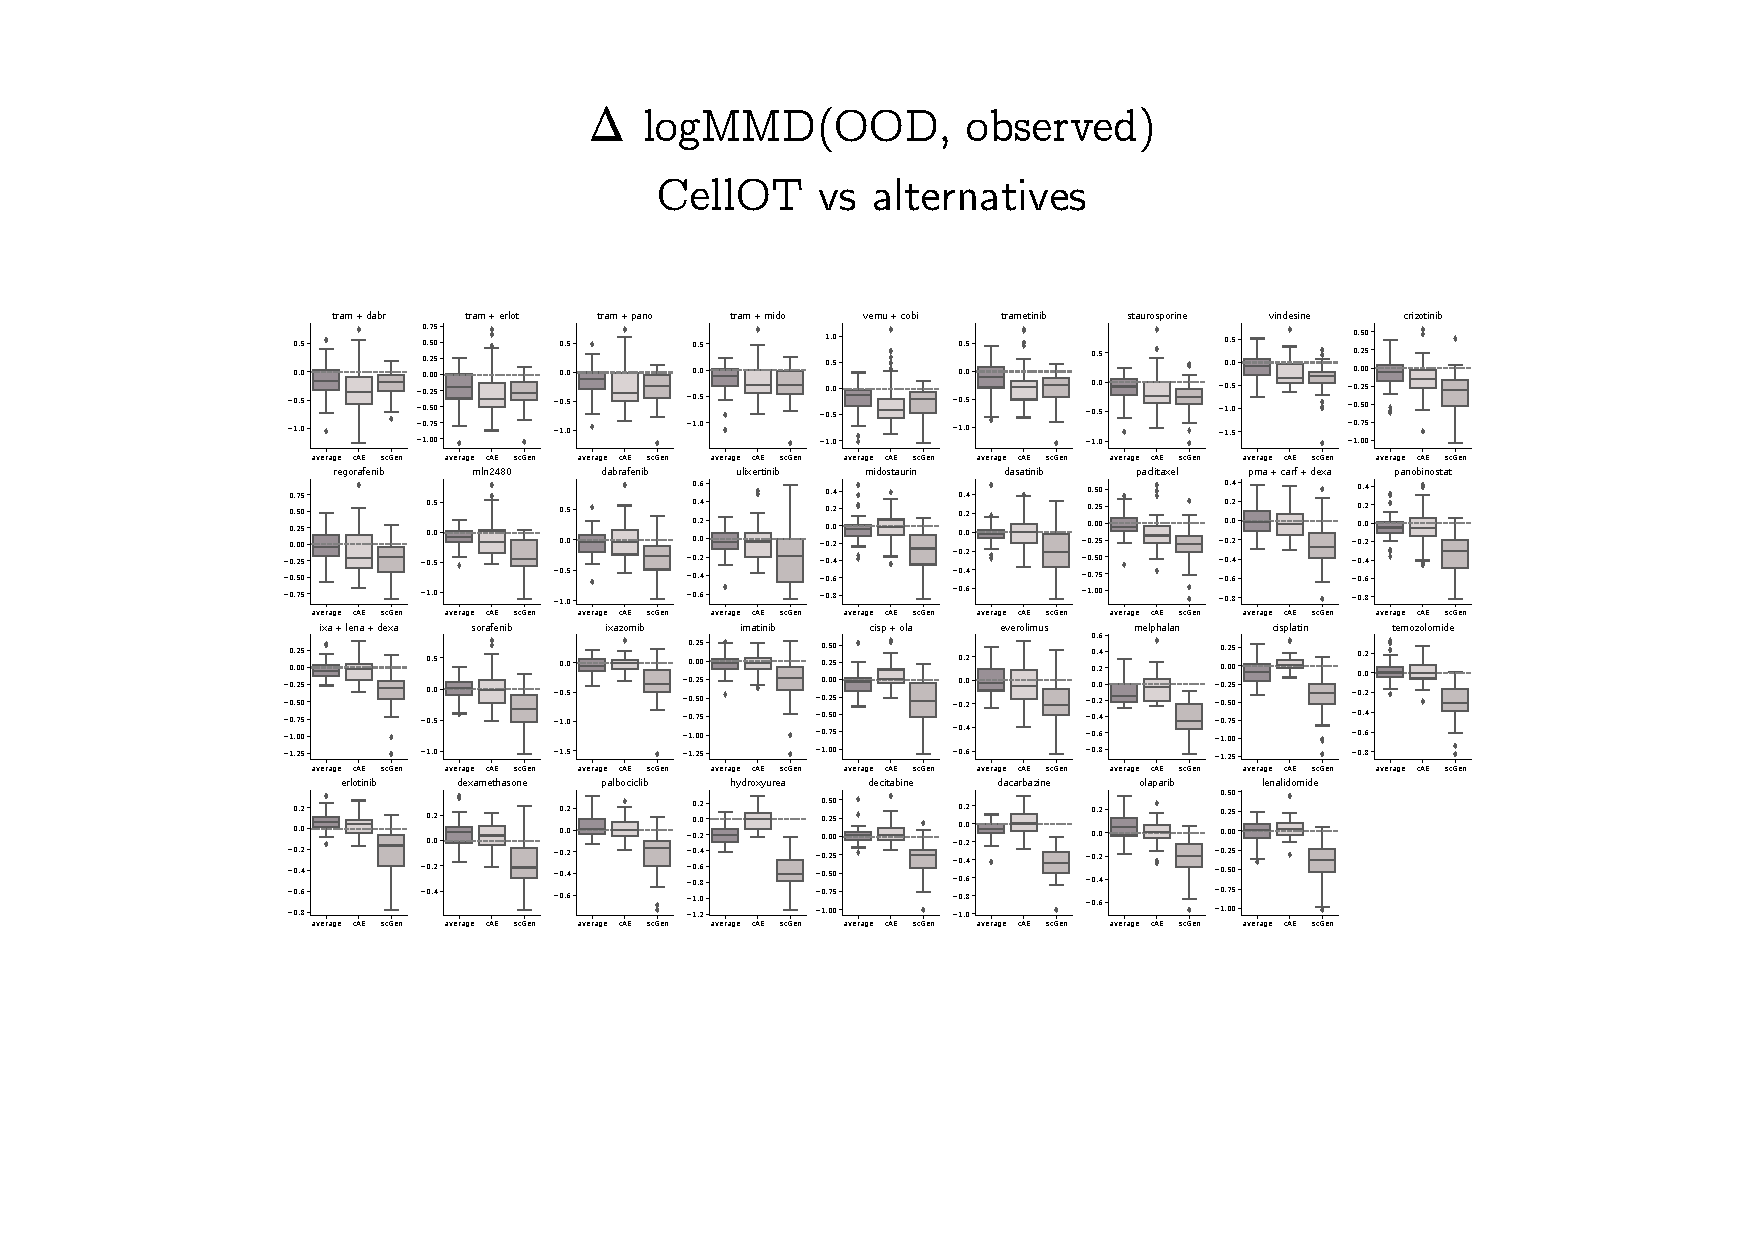
\includegraphics[width=0.95\textwidth]{figures/cellot-cohort/ood-eval-logmmd.pdf}
  \end{center}
  \caption{
    Pairwise logMMD differences comparing \textsc{CellOT} and baseline approaches.
    For each (drug, patient) pair, models are trained on the entire cohort with that patient held out.
    Each model predicts the drug response of the heldout patient
    and logMMD values are computed between the distribution of predicted treated states and the true treated states.
    Negative values correspond to settings where \textsc{CellOT} improves over the corresponding baseline.
  }
\label{fig:ood-eval-logmmd}
\end{figure}

\begin{figure}[h]
  \begin{center}
    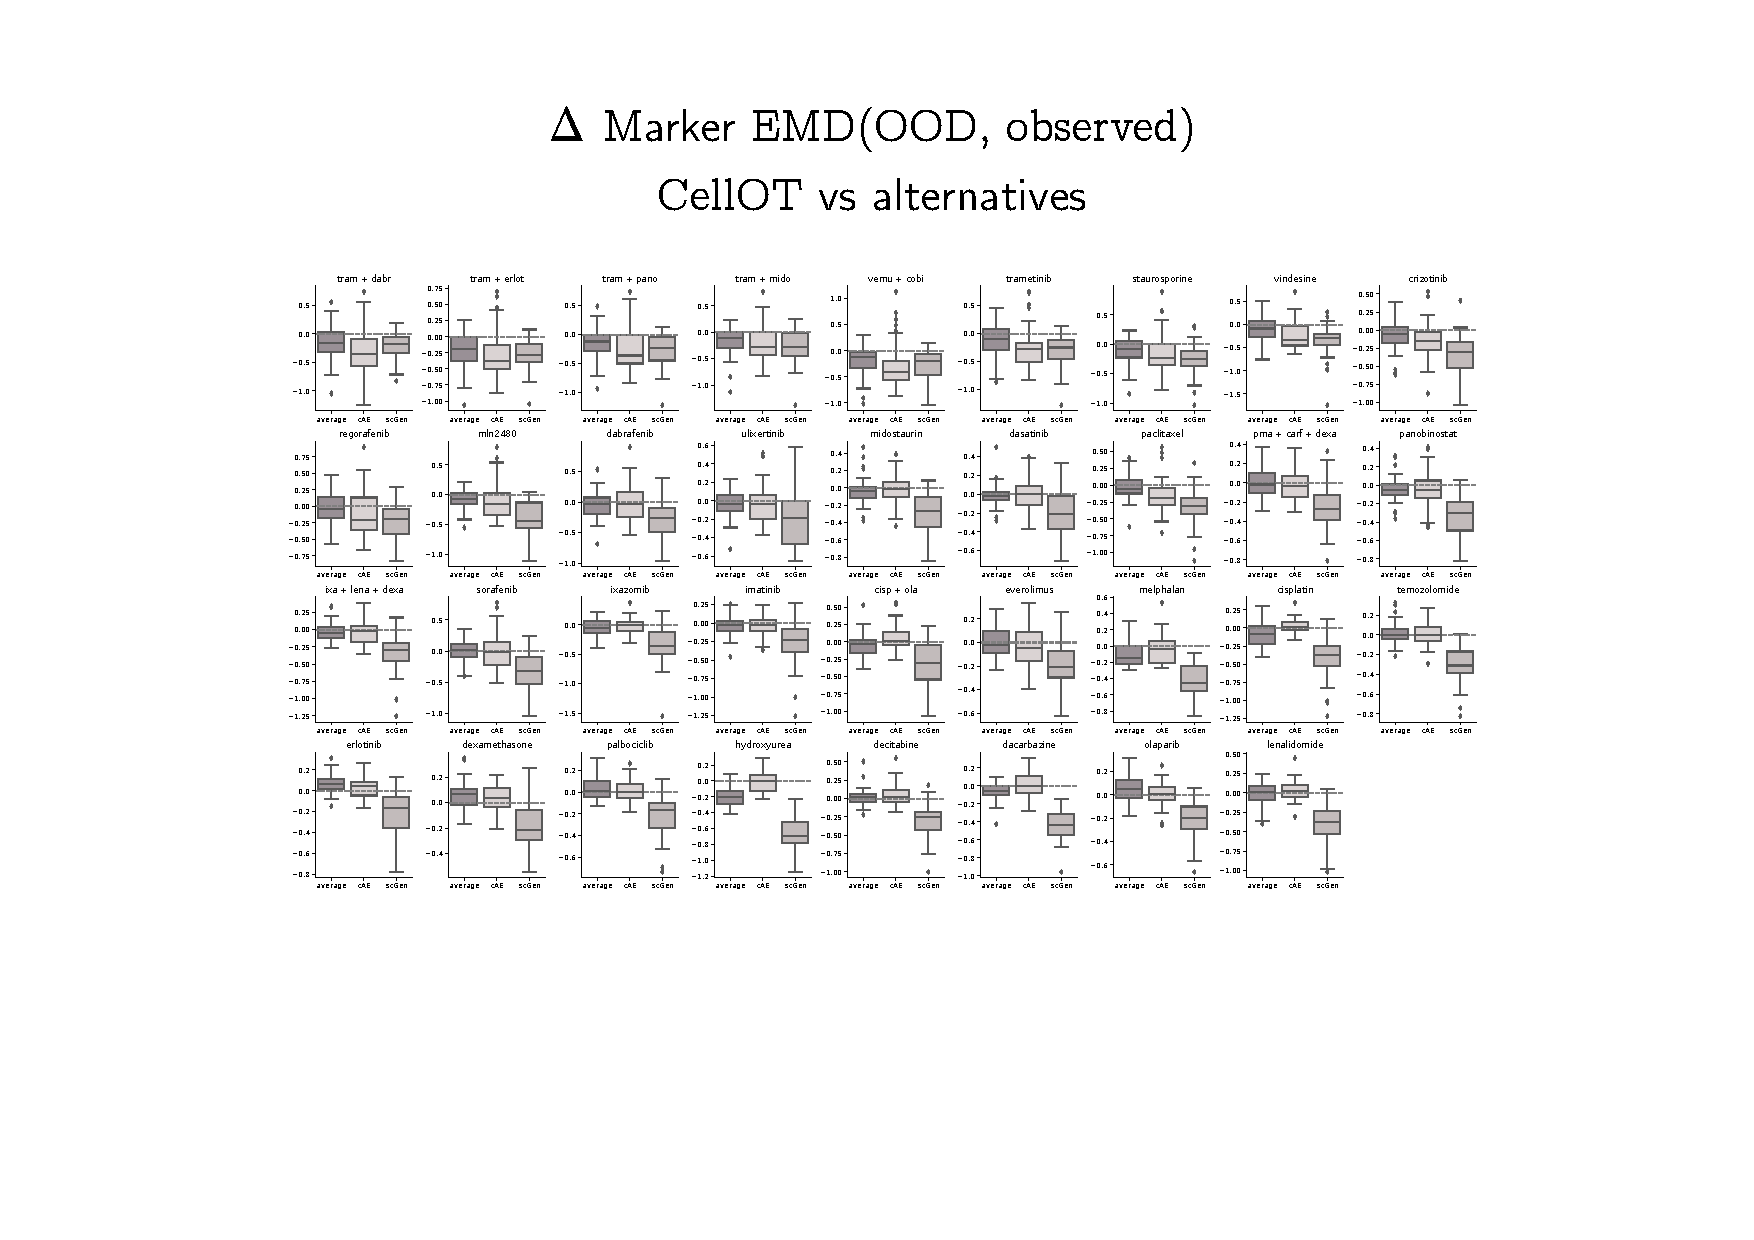
\includegraphics[width=0.95\textwidth]{figures/cellot-cohort/ood-eval-marker.pdf}
  \end{center}
  \caption{
    Pairwise marker EMD differences comparing $\textsc{CellOT}$ and baseline approaches.
    For each (drug, patient) pair, models are trained on the entire cohort with that patient held out.
    Each model predicts the drug response of the heldout patient
    and marker EMD values are computed between the distribution of predicted treated states and the true treated states.
    Negative values correspond to settings where $\textsc{CellOT}$ improves over the corresponding baseline.
  }
  \label{fig:ood-eval-marker}
\end{figure}

\begin{figure}
  \begin{center}
    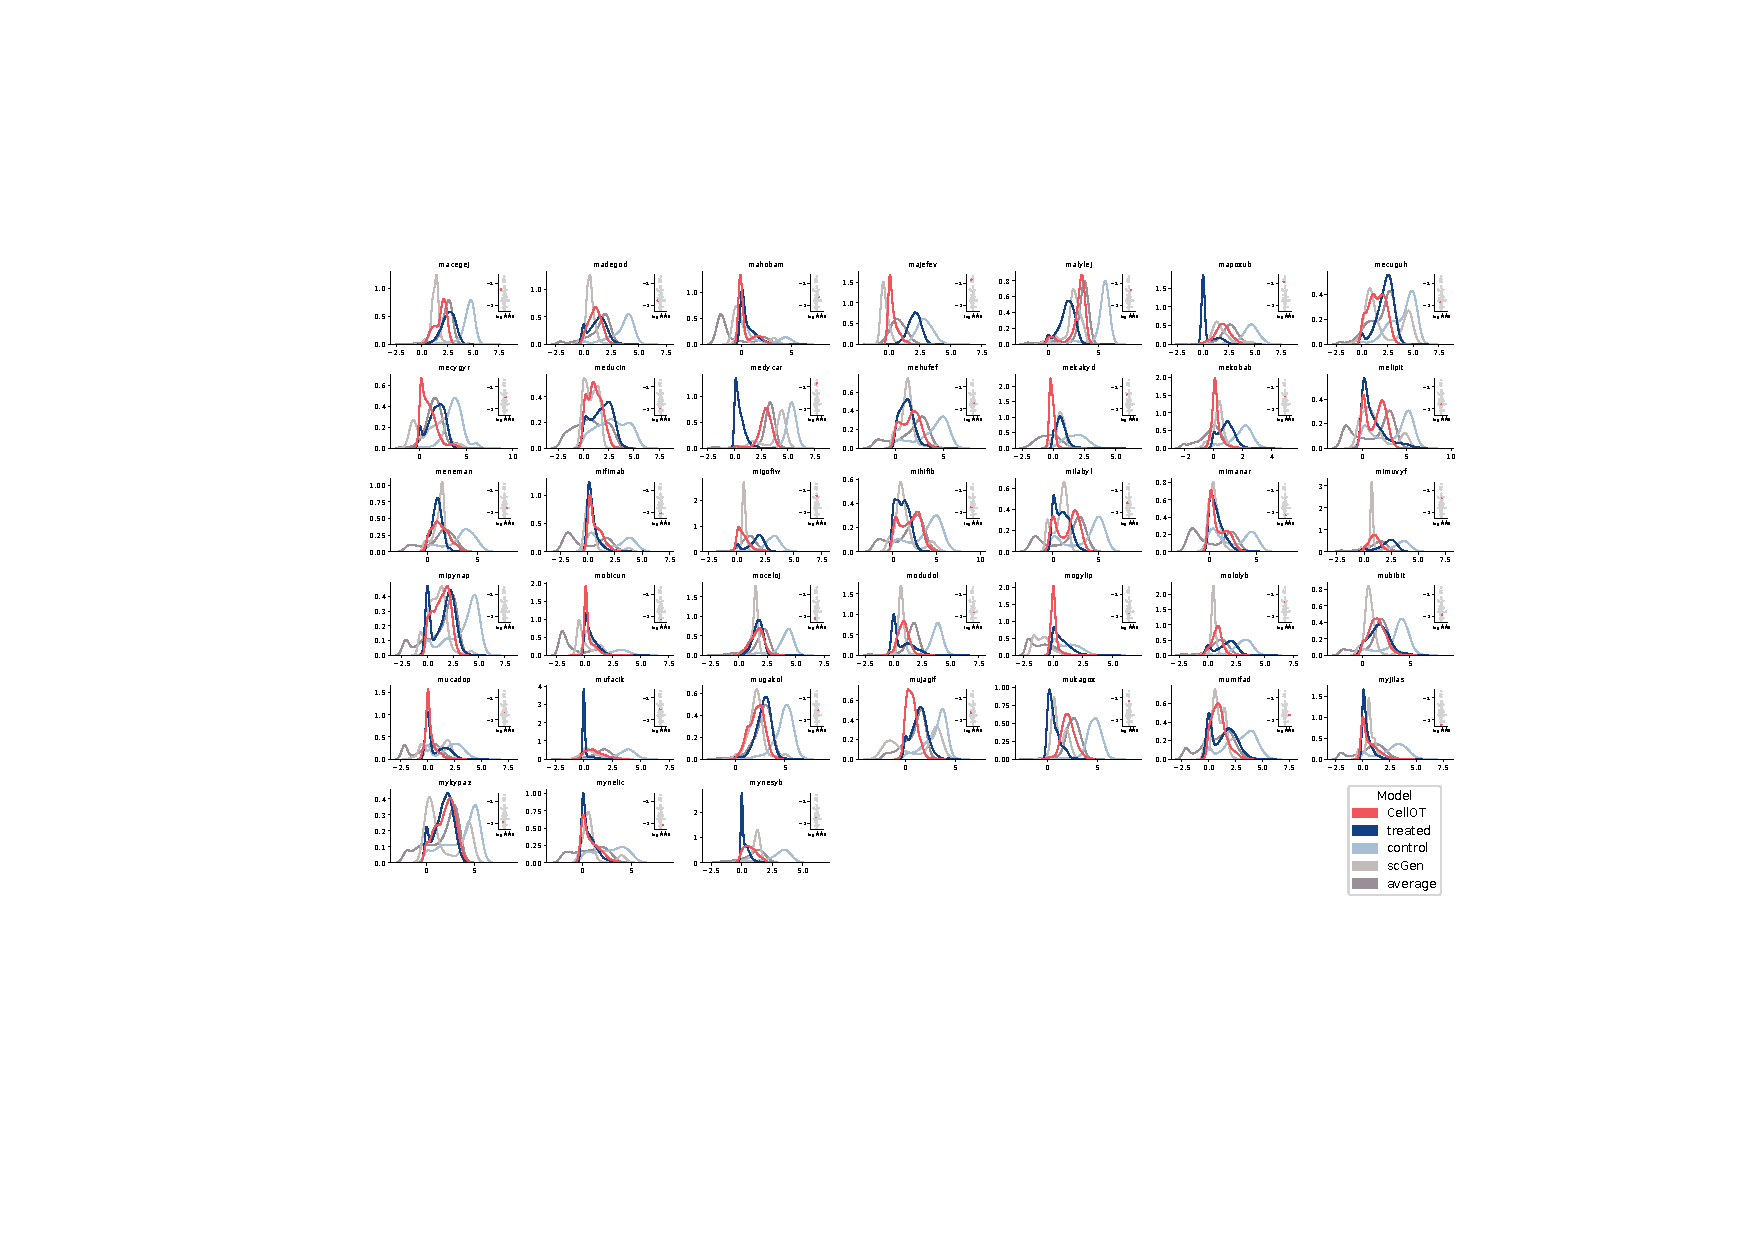
\includegraphics[width=0.95\textwidth]{figures/cellot-cohort/ood-predict-marginals.pdf}
  \end{center}
  \caption{
    Predicted response to trametinib dabrafenib combination treatment of each heldout samples.
    Marginals are shown for the treatment's marker feature, pERK.
    The inlay shows the selected heldout sample's logMMD score against the rest of the cohort.
  }\label{fig:ood-predict-marginals}
\end{figure}

\begin{figure}
  \begin{center}
    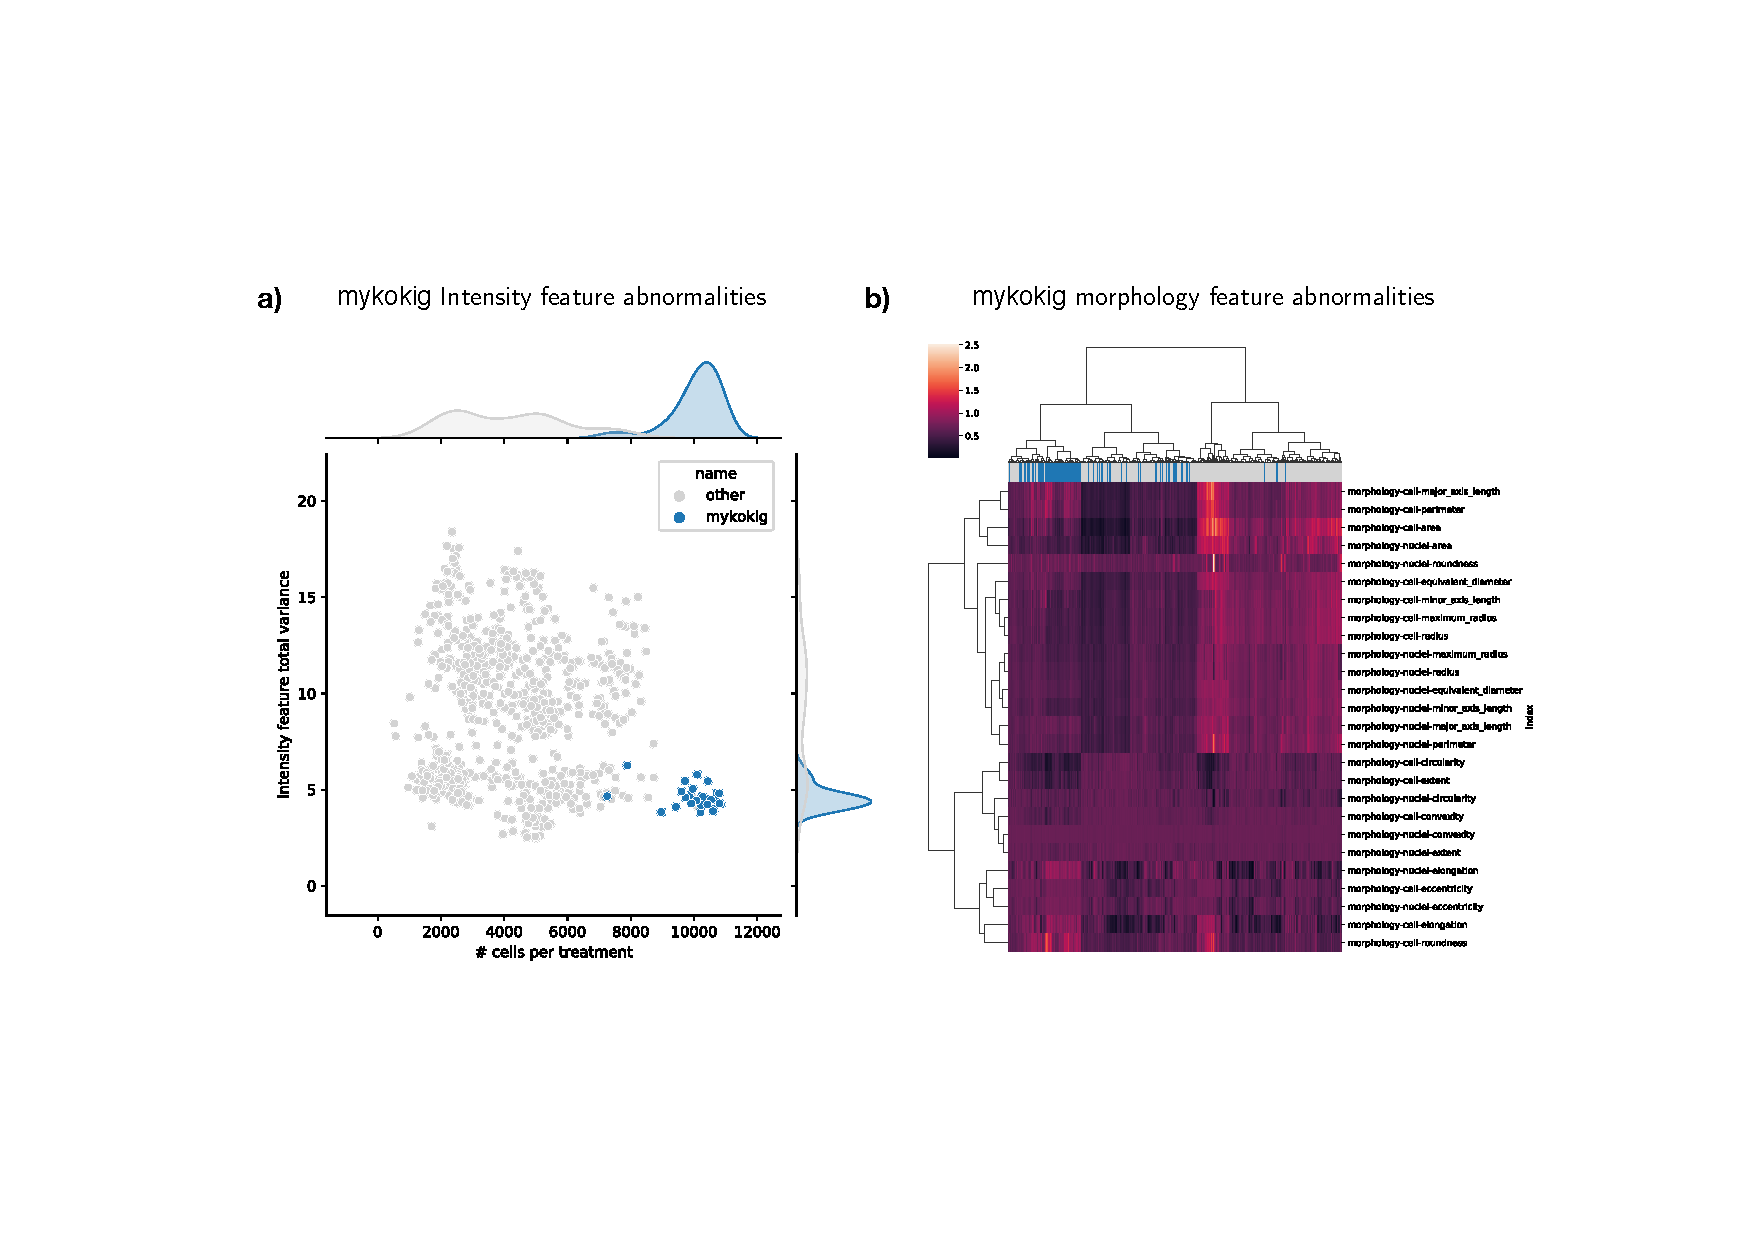
\includegraphics[width=0.95\textwidth]{figures/cellot-cohort/progression-exclude-mykokig.pdf}
  \end{center}
  \caption{
    Sample mykokig exhibits evidence for low quality cell segmentation and is removed from the progression prediction task.
  a) Scatter plot of number of treated cells by the variance of intensity features.  Each dot corresponds to a (treatment, sample) pair and treatments of mykokig are shown in blue. Mykokig behaves as an outlier as it has much more cells per treatment than other samples and these cells have low variance in their intensity features.
  b) Morphology features of mykokig cells indicate the presence of artifacts. The cluster map shows the distribution of each extracted morphology feature (rows) for cells sampled from mykokig and a subset of 5 samples from the full cohort. A large fraction of mykokig cells exhibit a strange unique morphology pattern of small round cells.
  }\label{fig:progression-exclude-mykokig}
\end{figure}

\begin{figure}
  \begin{center}
    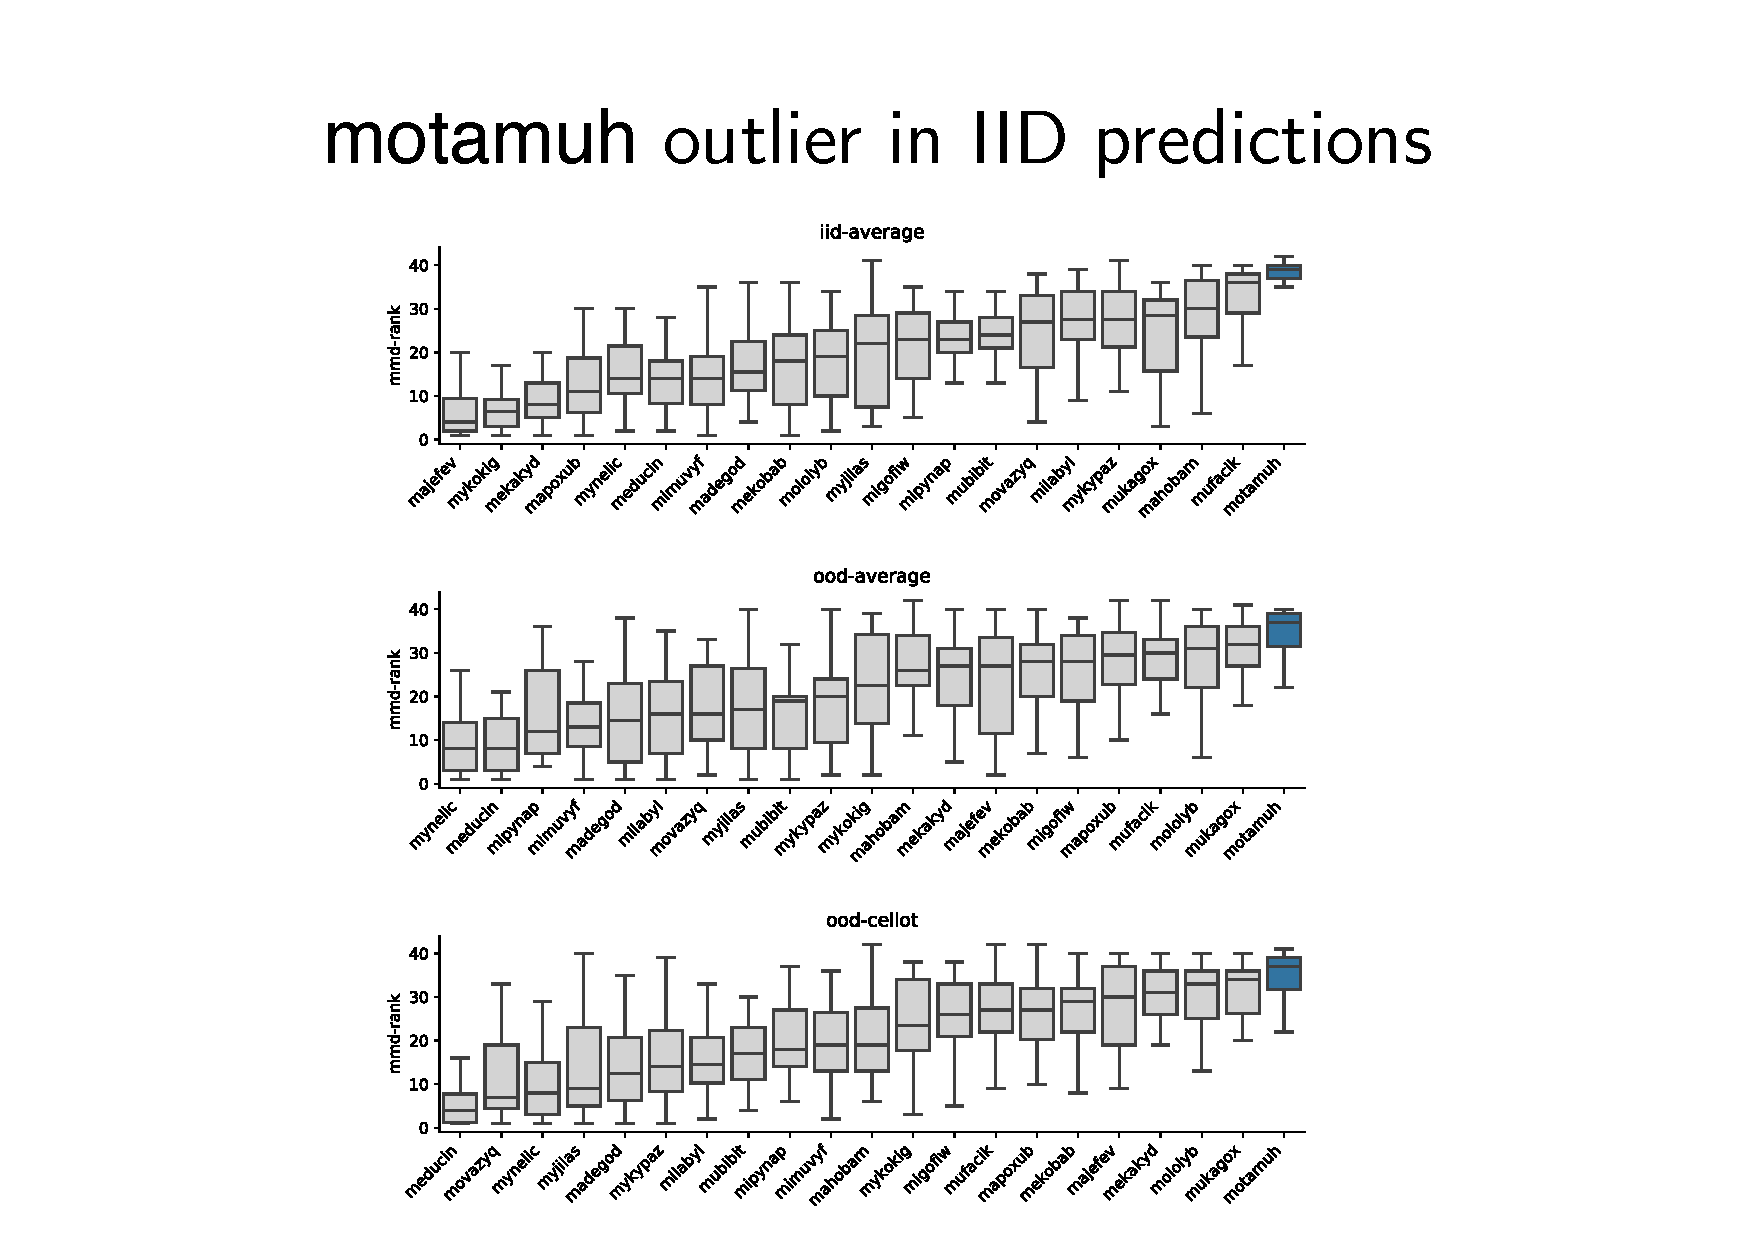
\includegraphics[width=0.95\textwidth]{figures/cellot-cohort/progression-exclude-motamuh.pdf}
  \end{center}
  \caption{
    The predicted responses for sample motamuh are consistently poor and the sample is therefore removed from the progression prediction task.
    Boxplots show the ranked MMD metric computed between each model's prediction and observed treated states for drugs considered in the progression prediction task.
    Results for the average model are shown in the IID and OOD setting as well as CellOT predictions in the OOD setting.
    Sample motamuh consistently ranks worst across all samples in the cohort for these prediction tasks.
  }\label{fig:progression-exclude-motamuh}
\end{figure}



%%%%%%%%%%%%%%%%%%%%%%%%%%%%%%%%%%%%%%%%%%
%% LIST OF TABLES / FIGURES / ALGORITHMS %
%%%%%%%%%%%%%%%%%%%%%%%%%%%%%%%%%%%%%%%%%%
\pdfbookmark[-1]{Lists of Tables}{lot}
\phantomsection\addcontentsline{toc}{chapter}{\listtablename}
\listoftables{}
\cleardoublepageempty{}
% \listsubcaptions
\pdfbookmark[-1]{Lists of Figures}{lof}
\phantomsection\addcontentsline{toc}{chapter}{\listfigurename}
\listoffigures{}
\cleardoublepageempty{}
\pdfbookmark[-1]{Lists of Algorithms}{loa}
%\phantomsection\addcontentsline{toc}{chapter}{\listalgorithmname}
%\listofalgorithms{}
\cleardoublepageempty{}


%%%%%%%%%%%%%%%%%
%% BIBLIOGRAPHY %
%%%%%%%%%%%%%%%%%
\let\l\relax
\phantomsection\addcontentsline{toc}{chapter}{\bibname}
\pdfbookmark[-1]{Bibliography}{book:bibliography}
\printbibliography{}
\cleardoublepageempty{}
\clearpage
\cleardoublepageempty{}
\end{document}
